\documentclass[12pt]{standalone}
\usepackage{tikz, amssymb} 
%\usetikzlibrary{calc, arrows.meta, decorations.pathreplacing}

\newcommand{\fourdots}{
  \fill (0,0) circle[radius=3.5pt];
  \fill (0,1) circle[radius=3.5pt];
  \fill (1,0) circle[radius=3.5pt];
  \fill (1,1) circle[radius=3.5pt];
}

\begin{document}

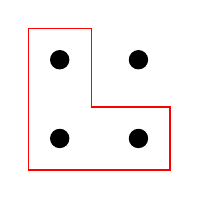
\begin{tikzpicture}[scale=1]

  \fourdots
  \draw[red] (-0.4, -0.4) -- (-0.4, 1.4) -- (0.4, 1.4) -- 
              (0.4, 0.4) -- (1.4, 0.4) -- (1.4, -0.4) -- 
              (0.4, -0.4) -- cycle;

\end{tikzpicture}

\end{document}
